\documentclass[article,colorback,accentcolor=tud4c]{tudreport}
% \usepackage{ngerman}

\usepackage[stable]{footmisc}
\usepackage{hyperref}

\usepackage{longtable}
\usepackage{multirow}
\usepackage{booktabs}

% \hypersetup{%
%   pdftitle={Eclipse Plug-in Development},
%   pdfauthor={Leo Roos},
%   pdfsubject={Beispieltext},
%   pdfview=FitH,
%   pdfstartview=FitV
% }

% \setcounter{seclinedepth}{1}
% 
% %%% Zum Tester der Marginalien %%%
%   \newif\ifTUDmargin\TUDmarginfalse
%   %%% Wird der Folgende Zeile einkommentiert,
%   %%% werden Marginalien gesetzt.
%   % \TUDmargintrue
%   \ifTUDmargin\makeatletter
%     \TUD@setmarginpar{2}
%   \makeatother\fi
% %%% ENDE: Zum Tester der Marginalien %%%
% 
% \newlength{\longtablewidth}
% \setlength{\longtablewidth}{0.7\linewidth}
% \addtolength{\longtablewidth}{-\marginparsep}
% \addtolength{\longtablewidth}{-\marginparwidth}


% \settitlepicture{tudreport-pic}
% \printpicturesize

\newcommand\tiger{%
  \textsc{TigersEye}
}


\newcommand\versionnum{%
  \texttt{0.0.1}
}

\newcommand\version{%
  v. \versionnum
}

\title{\tiger \version \\User Manual}
\subtitle{Leo Roos}
\subsubtitle{\href{mailto:leo\_roos@rbg.informatik.tu-darmstadt.de}{leo\_roos@rbg.informatik.tu-darmstadt.de}}
\institution{Department of Computer Science\\Advisor: Tom Dinkelaker}

\begin{document}
\maketitle
\begin{abstract}
  The \tiger Eclipse Plug-in is an IDE that strives to support easy creation of EDSLs. This guide describes how to install  \tiger for development, the different features and shows on some examples typical workflows.
\end{abstract}  

\tableofcontents
%\part{Lorem Ipsum (\textbackslash part)\label{part_lorem}}

  \section{Introduction}
	This guide will provide an overview over the implemented \tiger feature. \tiger has been previously known as \texttt{Popart}. The used examples are mostly adjusted versions of prior established work from Yevgen Fanshil[Reference1], Leonid Melnyk [Reference1], Thorsten Pater [Ref2] and David Marx[Ref2].
	I will describe the installation process. The implemented features and give examples for typical workflows.

  \section{Installation for Development}
	
	The \tiger plug-in itself consists of multiple separate plug-ins and has further dependencies to other plug-ins and libraries. It uses classes and extensions from the Groovy Plug-in and  Eclpse's JDT plug-ins, makes some use of different \texttt{apache.commons} libraries and uses further libraries to process code. It's core dependency is the used preprocessor \texttt{parlex}. Listing \ref{lst:dependencies} shows the necessary plug-ins and the required version if any.
	
	\begin{table}
	\center
	  \begin{tabular}{l|l|p{.4\textwidth}}
		Plug-in name & Version & Description\\ \hline
		Groovy Eclipse Feature & 2.1.1 & Groovy Eclipse Plug-in with version that is known to be compatible.\\
		org.apache.commons.io & - & Apache IO utility classes.\\
		org.apache.commons.lang& - & Apache general language utility classes.\\
		org.apache.commons.collections & - & Apache utility classes for collections.\\
		org.apache.log4j & [1.2 - 1.3) & Employed logging framework.\\
		slf4j-log4j12 & - & Employed logging facade with log4j binding.\\
		parlex & - & Preprocessor, performing the transformations. \\
		de.tud.stg.tigerseye & \versionnum & (Re)Exports commonly used libraries and plug-ins.\\
		de.tud.stg.tigerseye.eclipse.core & \versionnum & Core functionality.\\
		de.tud.stg.tigerseye.eclipse.ui& \versionnum & User Interface functionality.\\		
	  \end{tabular}
	\caption{Necessary Plug-ins}\label{lst:dependencies}
	\end{table}

	Once all the necessary plug-ins have been installed the \tiger plug-in can be started using the predefined \texttt{Tigerseye\_IDE} launch, which is located in the core plug-in. 
	It is possible that depending on the used operating system this launch configuration has to be adjusted. Alternatively one can start a new Eclipse Plug-in configuration with all available plug-ins active.
	

  \section{Features}

	The current version of \tiger provides the fundamental functaionlities in order to be able to use it as a language workbench. New languages can easily be created and deployed. After a restart they can be used in projects that have the \tiger nature. A \tiger nature can easily be added and removed via a popup menu. The installed DSLs can be configured through the preference pages, as well as the employed transformations. The \tiger editor is an extended version of the Groovy editor and provides keyword coloring for keywords of installed and activated DSLs.
	
	\subsection{Preferences}
	The prefrence pages are an important part of \tiger, since they provide the configuration of registered DSLs. In the main prefrence page (Figure \ref{fig:prefs_main}) the output source folder can be adjusted. Registered languages can be configured on the languages preference page (Figure \ref{fig:prefs_languages}). There languages can be activated or deactivated. Only activated languages will be usable during production. The extensions, that indicate which Concrete DSL class is responsible for which files of the according extension can be adjusted in the \texttt{Extensions} column. When a DSL is selected its keywords are shown below in the \textit{Declared Keywords of Selected DSL} dialog. The transformations preference page provides the adjustment of used transformations for the specified resource or DSL (Figure \ref{fig:prefs_transformations}). For each resource and dsl different transformations might be provided. These can be configured using the \texttt{Select Transformations} dialog (Figure \ref{fig:prefs_transformations_selected}). The dialog also shows additional informations about the currently selected transformation in a closeable tray window. The \tiger editor provides keyword coloring for active DSLs. The colors can be configured using the Tigerseye Editor preference page (see Figure \ref{fig:prefs_editor}), where every DSL can be configured seperately and the general keyword coloring can be activated or deactivated.
	
	\begin{figure}
	  \centering
	  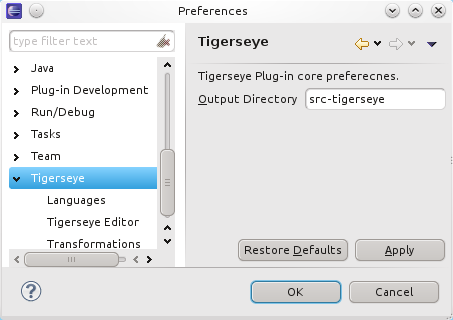
\includegraphics[scale=.5,keepaspectratio=true]{./pics/preferences_main.png}
	  % preferences_main.png: 453x320 pixel, 93dpi, 12.37x8.74 cm, bb=0 0 351 248
	  \caption{Tigerseye Main Preference Page}
	  \label{fig:prefs_main}
	\end{figure}

	\begin{figure}
	  \centering
	  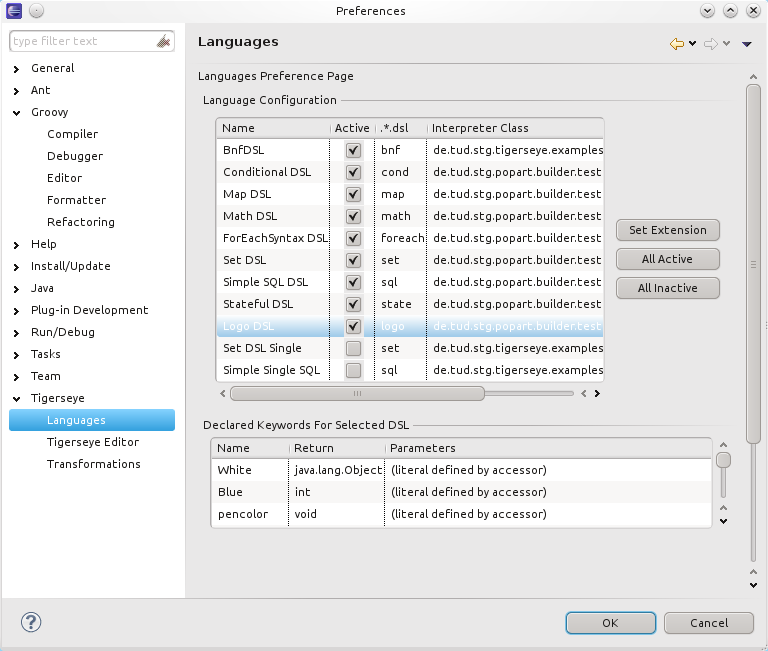
\includegraphics[scale=.5,keepaspectratio=true]{./pics/preferences_languages.png}
	  % preferences_main.png: 453x320 pixel, 93dpi, 12.37x8.74 cm, bb=0 0 351 248
	  \caption{Tigerseye Language Configuration Page}
	  \label{fig:prefs_languages}
	\end{figure}


	\begin{figure}
 \centering
 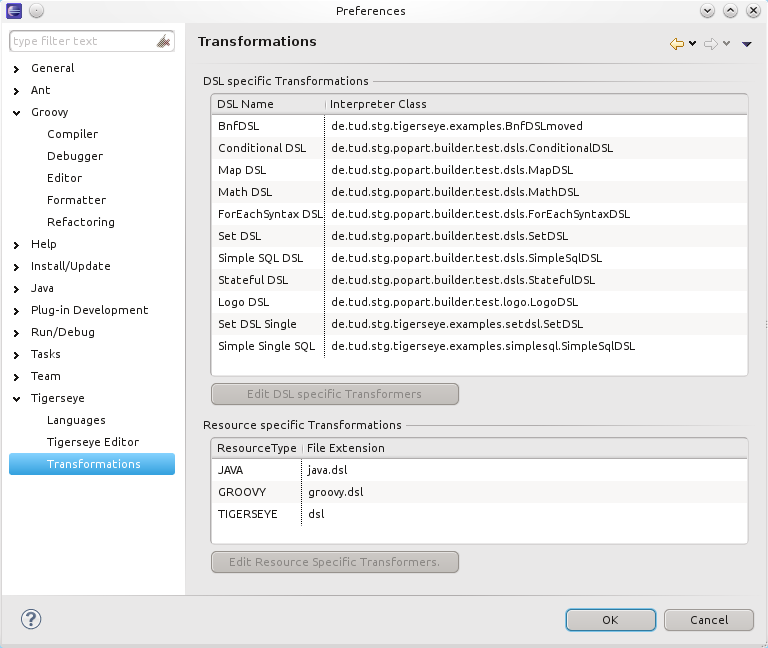
\includegraphics[scale=.5,keepaspectratio=true]{./pics/preferences_transformations.png}
 % preferences_main.png: 453x320 pixel, 93dpi, 12.37x8.74 cm, bb=0 0 351 248
 \caption{Tigerseye Transformations Preference Page}
 \label{fig:prefs_transformations}
\end{figure}


	\begin{figure}
 \centering
 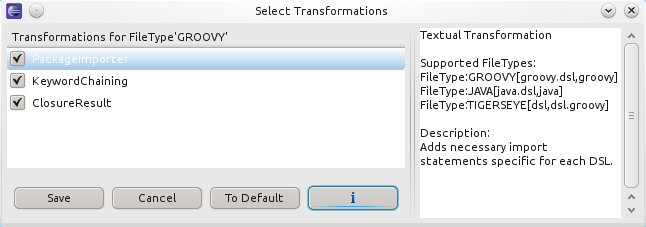
\includegraphics[scale=.5,keepaspectratio=true]{./pics/preferences_transformations_selected.png}
 % preferences_main.png: 453x320 pixel, 93dpi, 12.37x8.74 cm, bb=0 0 351 248
 \caption{Tigerseye Transformations Configuration}
 \label{fig:prefs_transformations_selected}
\end{figure}

	\begin{figure}
 \centering
 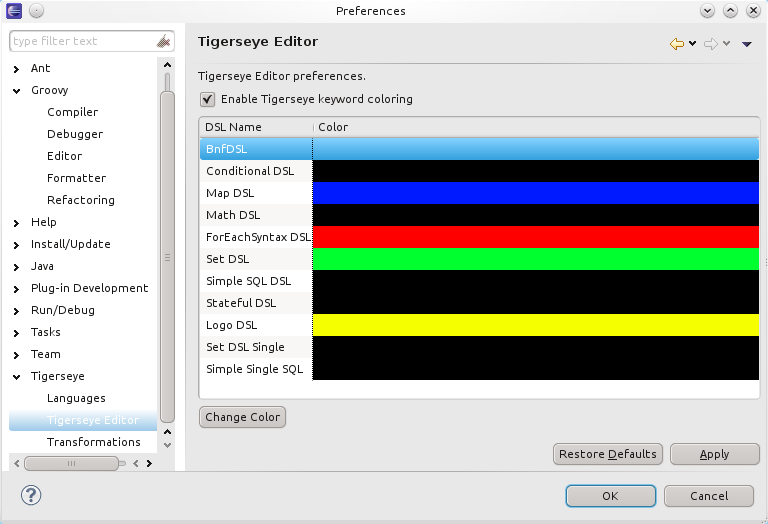
\includegraphics[scale=.5,keepaspectratio=true]{./pics/preferences_editor.png}
 % preferences_main.png: 453x320 pixel, 93dpi, 12.37x8.74 cm, bb=0 0 351 248
 \caption{Tigerseye Editor Preference Page}
 \label{fig:prefs_editor}
\end{figure}


	
	
	\subsection{Add and Remove \tiger Nature}
	  \tiger has additional requirements which will be imported when adding the \tiger nature to a project. The project must have at least the Java nature otherwise the transformation to a \tiger project is not possible. Figure \ref{fig:add_tiger_nature} shows the available popup menu to add the \tiger nature to a project. This will do two things. A seperate source folder will be created into which the translated DSL files will be output (\texttt{src-tigerseye}) and a new class path container will be added which contains the runtime libraries (\texttt{popartAnnotations.jar, popart.jar, edslNature.jar}) and the libraries of registered DSLs as well as their dependencies. For example \texttt{de.tud.stg.tigerseye.examples.LogoDSL} and \texttt{de.tud.stg.tigerseye.examples.DSLDefinitions}. 
	
	\begin{figure}
	  \centering
	  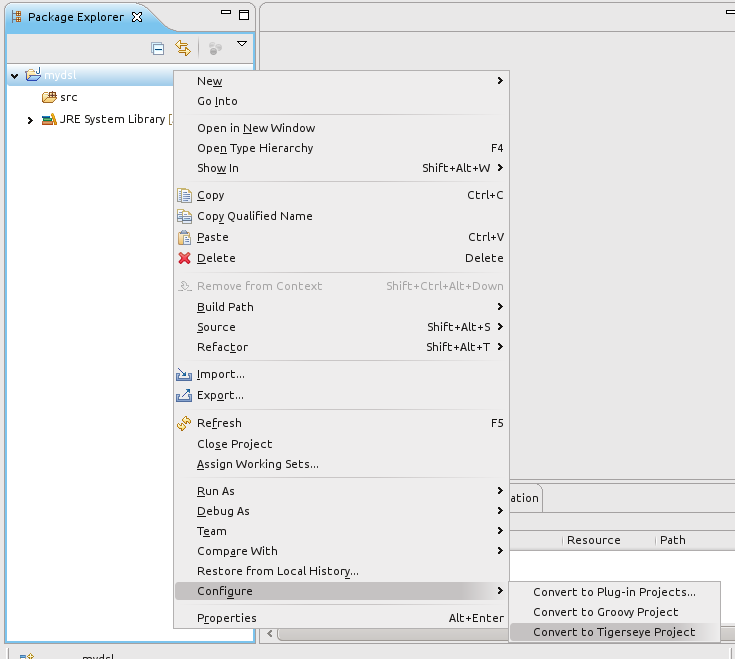
\includegraphics[width=.5\textwidth,keepaspectratio=true]{./pics/convert_to_tigerseye.png}
	  % new_tigesreye_language.png: 525x500 pixel, 93dpi, 14.34x13.66 cm, bb=0 0 406 387
	  \caption{Add the \tiger Nature to a Java Project}
	  \label{fig:add_tiger_nature}
	\end{figure}
	
	\begin{figure}
	  \centering
	  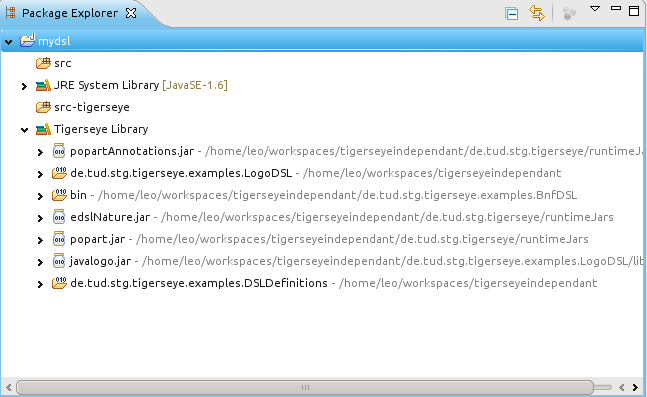
\includegraphics[width=.5\textwidth,keepaspectratio=true]{./pics/tigerseye_dependencies.png}
	  % new_tigesreye_language.png: 525x500 pixel, 93dpi, 14.34x13.66 cm, bb=0 0 406 387
	  \caption{\tiger Dependencies}
	  \label{fig:tiger_added_dependencies}
	\end{figure}
	
	\begin{figure}
	  \centering
	  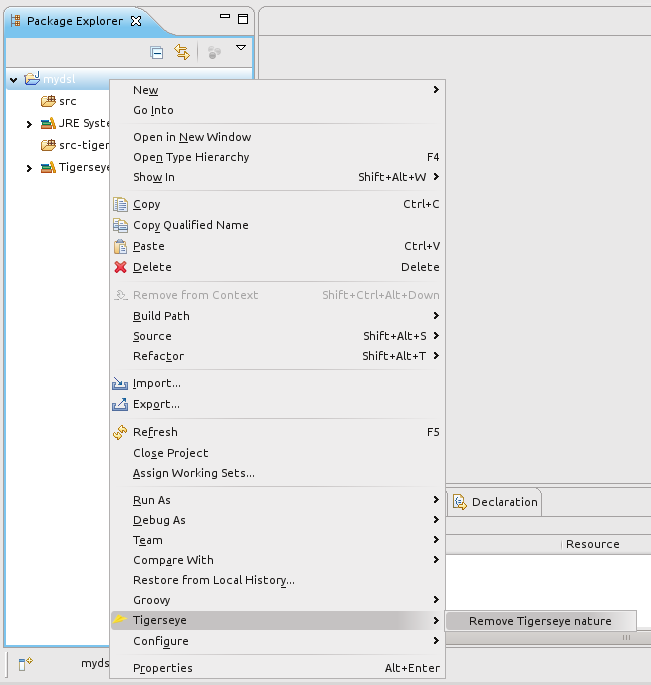
\includegraphics[width=.5\textwidth,keepaspectratio=true]{./pics/remove_tigerseye_nature.png}
	  % new_tigesreye_language.png: 525x500 pixel, 93dpi, 14.34x13.66 cm, bb=0 0 406 387
	  \caption{Remove the \tiger Nature from a Project}
	  \label{fig:remove_tiger_nature}
	\end{figure}
	
	\subsection{\tiger Language Definition Wizard}
	  A new language can be created using the \textit{New Language Wizard}. For that choose via the File -> New -> Other Dialog (Figure \ref{fig:new_tiger_lang}) the \textit{Tigerseye Language Definition} Wizard. Figure \ref{fig:tiger_lang_definition_page1} shows the first page of the Wizard. There the name of the main language class can be defined. As shown the default package is not a valid package for a language defintion since this will cause problems when trying to use the language within a Java class. Figure \ref{fig:tiger_lang_definition_page2} shows the actual language definition page. There the different literals, operations and structured elements can be added. How to use this page will be discussed in Section \ref{sec:examples}.
	
	\begin{figure}
	  \centering
	  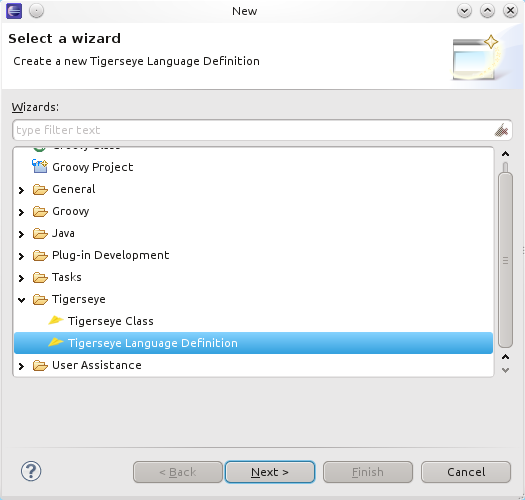
\includegraphics[width=.5\textwidth,keepaspectratio=true]{./pics/new_tigesreye_language.png}
	  % new_tigesreye_language.png: 525x500 pixel, 93dpi, 14.34x13.66 cm, bb=0 0 406 387
	  \caption{Choosing the New Tigerseye Language Wizard}
	  \label{fig:new_tiger_lang}
	\end{figure}

	\begin{figure}
	  \centering
	  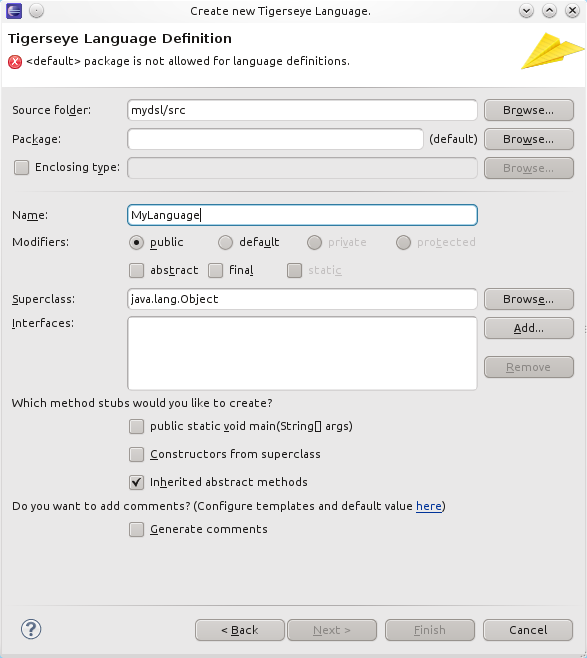
\includegraphics[width=.5\textwidth,keepaspectratio=true]{./pics/tigerseye_language_definition_page1.png}
	  % new_tigesreye_language.png: 525x500 pixel, 93dpi, 14.34x13.66 cm, bb=0 0 406 387
	  \caption{Tigerseye Language Definition Wizard Page 1}
	  \label{fig:tiger_lang_definition_page1}
	\end{figure}
	
	\begin{figure}
	  \centering
	  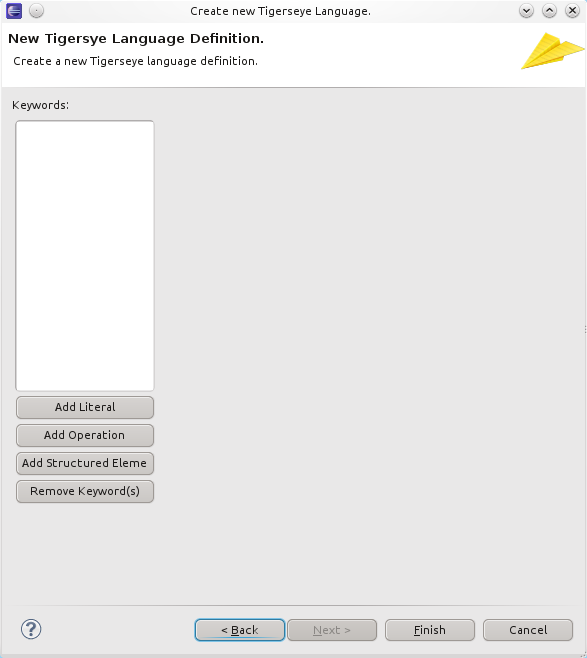
\includegraphics[width=.5\textwidth,keepaspectratio=true]{./pics/tigerseye_language_definition_page2.png}
	  % new_tigesreye_language.png: 525x500 pixel, 93dpi, 14.34x13.66 cm, bb=0 0 406 387
	  \caption{Tigerseye Language Definition Wizard Page 2}
	  \label{fig:tiger_lang_definition_page2}
	\end{figure}
	
	\subsection{New \tiger Class Wizard}
	  The new \tiger Class enables easy creation of new DSL classes. In Figure \ref{fig:new_tiger_class_page} the Wizard is shown. It is basically an adjusted version of the new Java Class Wizard. Additionally to being able to define the typical class properties a DSL can be chosen which one wishes to use in the class.

	\begin{figure}
	\centering
	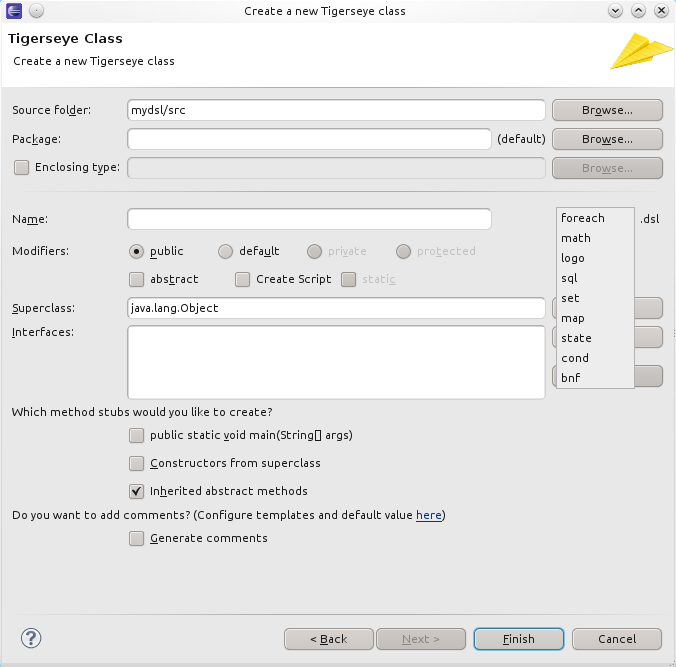
\includegraphics[scale=.5]{./pics/new_tigerseye_class_wizard.png}
	% new_tigerseye_class_wizard.png: 0x0 pixel, 300dpi, 0.00x0.00 cm, bb=
	\caption{New Tigerseye Class Wizard}
	\label{fig:new_tiger_class_page}
	\end{figure}	
	
	
	\subsection{Launch Tigerseye DSL}
	  A tigerseye DSL can be launched using the launch shortcut or via the \textit{Run Configurations Dialog}. Figure \ref{fig:launch_shortcut} shows a launch using a launch shortcut. Figure  \ref{fig:launch_run_configurations_dialog} shows the launch via the \emph{Run Configurations Dialog}. There one can adjust the default settings and choose the project from which a DSL will be launched as well as the dsl file to launch. When using the launch shortcut the Groovy default launch configuration is assumed which will set additional classpath properties. These can as well be adjusted using the Run Configurations dialog.
	
	\begin{figure}
 \centering
 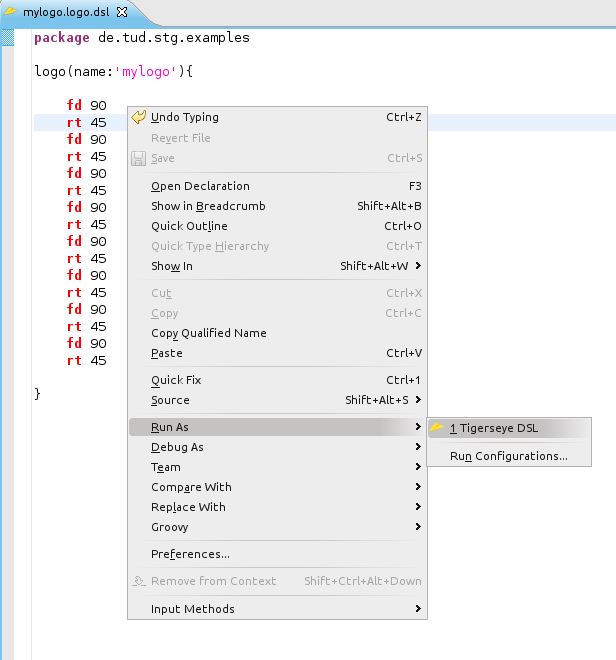
\includegraphics[scale=0.5]{./pics/launch_shortcut.png}
 % launch_shortcut.png: 616x660 pixel, 93dpi, 16.83x18.03 cm, bb=0 0 477 511
 \caption{Launch via Context Menu}
 \label{fig:launch_shortcut}
\end{figure}

\begin{figure}
 \centering
 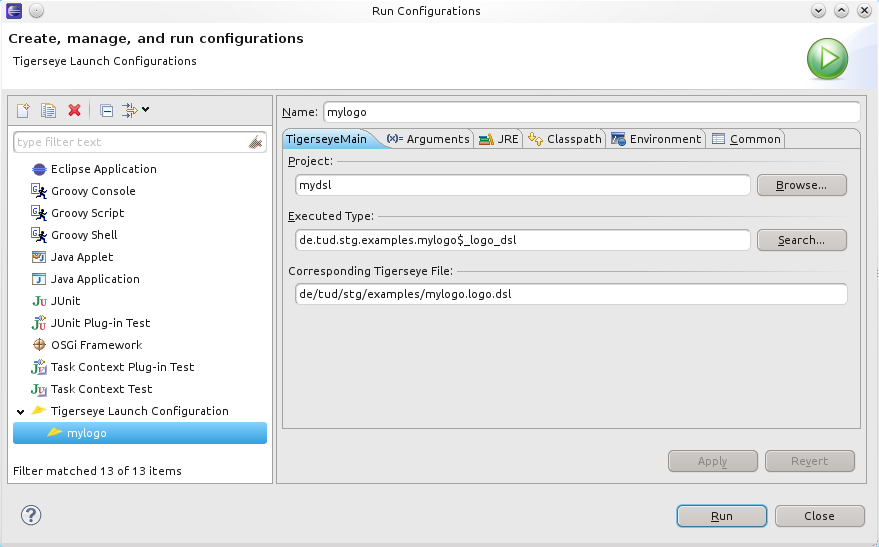
\includegraphics[scale=.5]{./pics/launch_run_configurations_dialog.png}
 % launch_run_configurations_dialog.png: 879x547 pixel, 93dpi, 24.01x14.94 cm, bb=0 0 681 424
 \caption{Launch via the Run Configurations Dialog}
 \label{fig:launch_run_configurations_dialog}
\end{figure}


	

  \section{Examples}\label{sec:examples}
  
  To clarify the usage 

In order to work with \tiger you need to create a project that has at least the Java nature (which will probably be a Java or Groovy project). Once you have a project you can create a new language using the \texttt{New Tigerseye Language} Wizard. 


  \appendix

  \listoffigures\addcontentsline{toc}{section}{\listfigurename}
\end{document}
